\documentclass[aspectratio=169]{beamer}

\usepackage{listings}
\definecolor{dkgreen}{rgb}{0,0.6,0}
\definecolor{gray}{rgb}{0.5,0.5,0.5}
\definecolor{mauve}{rgb}{0.58,0,0.82}

\usepackage{tikz}
\usetikzlibrary{matrix,fit,positioning,overlay-beamer-styles}

\lstdefinestyle{myScalastyle}{
  language=scala,
  aboveskip=2mm,
  belowskip=2mm,
  showstringspaces=false,
  columns=flexible,
  basicstyle={\small\ttfamily},
  numbers=none,
  numberstyle=\small\color{gray},
  keywordstyle=\color{blue},
  commentstyle=\color{dkgreen},
  stringstyle=\color{mauve},
  frame=single,
  breaklines=true,
  breakatwhitespace=true,
  tabsize=3,
}

\lstdefinestyle{myTerminal}{
  frame=tb,
  aboveskip=2mm,
  belowskip=2mm,
  showstringspaces=false,
  columns=flexible,
  basicstyle={\small\ttfamily},
  numbers=none,
  numberstyle=\small\color{gray},
  frame=single,
  breaklines=true,
  breakatwhitespace=true,
  tabsize=3,
}

\beamertemplatenavigationsymbolsempty

\title{Create custom linters using TASTy inspection}
\author{Vincent de Haan}
\date{}

\begin{document}

\frame{\maketitle}

\frame{
  \frametitle{Who am I?}

  \begin{itemize}
    \item self-employed Scala engineer
    \item with a background in both law and mathematics
    \item currently working on smart energy meters
  \end{itemize}
}

\frame{
  \frametitle{Goals for today}

  \begin{itemize}
    \item What is a TASTy?
    \item How to inspect it?
    \item How to create a custom linter?
  \end{itemize}
}

\begin{frame}[fragile]
  \frametitle{How does this work? (Scala 2) I}
  
  \begin{lstlisting}[style=myScalastyle,frame=none]
class Foo {
    def f(i: Int): Int = 1
    def g(implicit i: Int): Int = 2
}
  \end{lstlisting}
  \pause
  \begin{lstlisting}[style=myTerminal,frame=none]

> javap Foo   
Compiled from "Foo.scala"
public final class Foo {
  public static int g(int);
  public static int f(int);
}
  \end{lstlisting}
  
\end{frame}

\begin{frame}[fragile]
  \frametitle{How does this work? (Scala 2) II}

  \begin{lstlisting}[style=myScalastyle,frame=none]
object FooClient {
    implicit val i: Int = 3
    
    Foo.g
    Foo.f // Does not compile
}
  \end{lstlisting}
  
  \pause
 
  How does the compiler know \texttt{g} takes an implicit?
\end{frame}

\begin{frame}[fragile]
  \frametitle{How does this work? (Scala 2) III}
  
  \begin{lstlisting}[style=myTerminal,frame=none]

javap -v Foo
...
RuntimeVisibleAnnotations:
  0: #6(#7=s#8)
    scala.reflect.ScalaSignature(
      bytes="\u0006\u0005}9Q!\u0002\u0004\t\u0002%1Qa\u0003
      \u0004\t\u00021AQaE\u0001\u0005\u0002QAQ!F\u0001\u0005
      \u0002YAQ\u0001H\u0001\u0005\u0002u\t1AR8p\u0015\u00059
      \u0011a\u0002\u001ff[B$\u0018PP\u0002\u0001!\tQ\u0011!D
     ..."
    )
  ScalaSig: length = 0x3 (unknown attribute)
   05 02 00
  \end{lstlisting}

\end{frame}

\begin{frame}[fragile]
  \frametitle{How does this work? (Scala 2) IV}
  

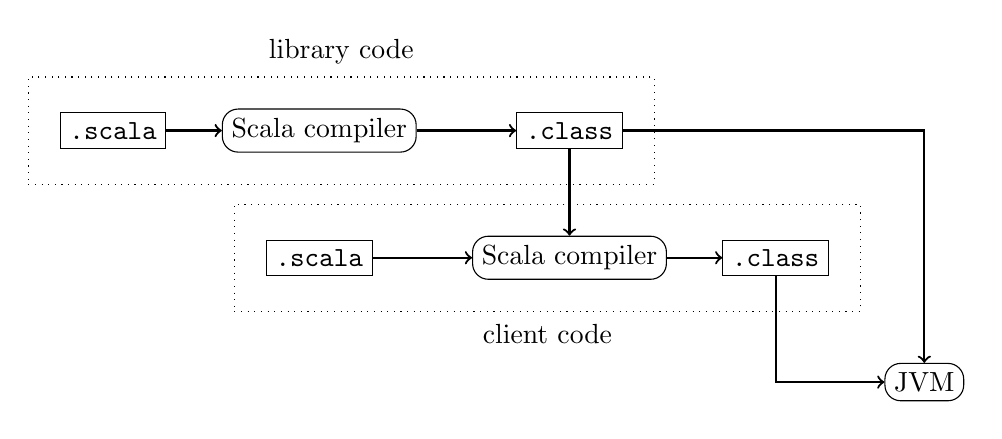
\begin{tikzpicture}
  \matrix [row sep=3em,
    column sep=2em]{
    \node (src1) [draw, shape=rectangle] {\texttt{.scala}}; &
  \node (cmp1) [draw, shape=rectangle, rounded corners=2mm] {Scala compiler}; &
  \node (cls1) [draw, shape=rectangle] {\texttt{.class}};\\
  & \node (src2) [draw, visible on=<2->, shape=rectangle] {\texttt{.scala}}; &
  \node (cmp2) [draw, visible on=<2->, shape=rectangle, rounded corners=2mm] {Scala compiler}; &
   \node (cls2) [draw, visible on=<2->, shape=rectangle] {\texttt{.class}};\\
   & & & & \node (jvm) [draw, visible on=<3->, shape=rectangle, rounded corners=2mm] {JVM}; \\};
  \draw[->, thick] (src1) -- (cmp1);
  \draw[->, thick] (cmp1) -- (cls1);
  \visible<2->{\draw[->, thick] (src2) -- (cmp2);
  \draw[->, thick] (cmp2) -- (cls2);
  \draw[->, thick] (cls1) -- (cmp2);
  \node (box2) [dotted, fit=(src2)(cmp2)(cls2), draw, inner sep=4mm] {};
  \node at (box2.south) [below, inner sep=1.5mm] {client code}; }
  \visible<3->{\draw[->, thick] (cls1) -| (jvm);
  \draw[->, thick] (cls2) |- (jvm);}
  \node (box1) [dotted, fit=(src1)(cmp1)(cls1), draw, inner sep=4mm] {}; 
  \node at (box1.north) [above, inner sep=1.5mm] {library code};
\end{tikzpicture}

  
\end{frame}

\begin{frame}[fragile]
\frametitle{How about Scala 3?}

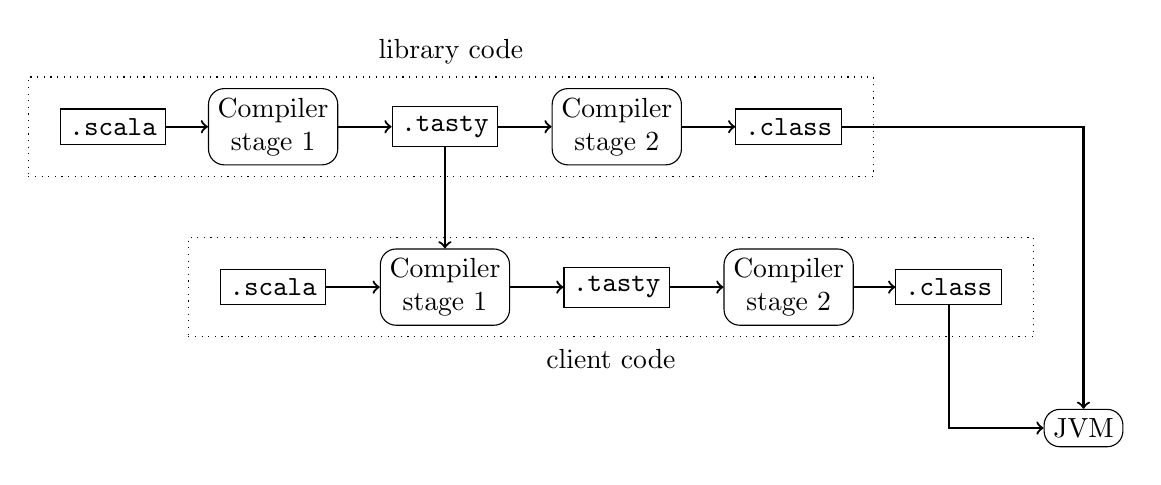
\begin{tikzpicture}
  \matrix[row sep=3em, column sep=1.5em,nodes={align=center}]{
    \node (src1) [draw, shape=rectangle] {\texttt{.scala}}; &
    \node (cmp11) [draw, shape=rectangle, rounded corners=2mm] {Compiler\\stage 1}; &
    \node (tst1) [draw, shape=rectangle] {\texttt{.tasty}}; &
    \node (cmp12) [draw, shape=rectangle, rounded corners=2mm] {Compiler\\stage 2}; &
    \node (cls1) [draw, shape=rectangle] {\texttt{.class}};\\
    & \node (src2) [draw, shape=rectangle, visible on=<2->] {\texttt{.scala}}; &
    \node (cmp21) [draw, shape=rectangle, rounded corners=2mm, visible on=<2->] {Compiler\\stage 1}; &
    \node (tst2) [draw, shape=rectangle, visible on=<2->] {\texttt{.tasty}}; &
    \node (cmp22) [draw, shape=rectangle, rounded corners=2mm, visible on=<2->] {Compiler\\stage 2}; &
    \node (cls2) [draw, shape=rectangle, visible on=<2->] {\texttt{.class}};\\
   & & & & & & \node (jvm) [draw, visible on=<3->, shape=rectangle, rounded corners=2mm, visible on=<3->] {JVM}; \\
  };
  \draw[->, thick] (src1) -- (cmp11);
  \draw[->, thick] (cmp11) -- (tst1);
  \draw[->, thick] (tst1) -- (cmp12);
  \draw[->, thick] (cmp12) -- (cls1);
  \visible<2->{
    \draw[->, thick] (src2) -- (cmp21);
    \draw[->, thick] (cmp21) -- (tst2);
    \draw[->, thick] (tst2) -- (cmp22);
    \draw[->, thick] (cmp22) -- (cls2);
    \draw[->, thick] (tst1) -- (cmp21);
    \node (box2) [dotted, fit=(src2)(cls2), draw, inner sep=4mm] {}; 
    \node at (box2.south) [below, inner sep=1.5mm] {client code};
  }
  \visible<3->{
    \draw[->, thick] (cls1) -| (jvm);
    \draw[->, thick] (cls2) |- (jvm);
  }
  \node (box1) [dotted, fit=(src1)(cls1), draw, inner sep=4mm] {}; 
  \node at (box1.north) [above, inner sep=1.5mm] {library code};

\end{tikzpicture}
\end{frame}

\begin{frame}[fragile]
\frametitle{Can we inspect these \texttt{.tasty} files?}
\pause
Yes!
\pause
\begin{lstlisting}[style=myScalastyle,frame=none]
import scala.quoted.*
import scala.tasty.inspector.*

class MyInspector extends Inspector:
   def inspect(using Quotes)(tastys: List[Tasty[quotes.type]]): Unit =
      import quotes.reflect.*
      for tasty <- tastys do
         val tree = tasty.ast
         // Do something with the tree
\end{lstlisting}
\pause
\begin{lstlisting}[style=myScalastyle,frame=none]
         println(tree)
\end{lstlisting}

\end{frame}

\begin{frame}[fragile]
\frametitle{A simple example}
\begin{columns}
\begin{column}{0.4\textwidth}
\begin{lstlisting}[style=myScalastyle,frame=none]
object TestApp extends App {
  println("Hello world!")
}
\end{lstlisting}
\end{column}
\pause
\begin{column}{0.6\textwidth}
  \begin{lstlisting}[style=myTerminal,frame=none]
PackageDef(Ident(example),List(ValDef(TestApp,
Ident(TestApp$),Apply(Select(New(Ident(
TestApp$)),<init>),List())), TypeDef(
TestApp$,Template(DefDef(<init>,List(List()),
TypeTree[TypeRef(TermRef(ThisType(
TypeRef(NoPrefix,module class <root>)),
object scala),Unit)],EmptyTree),List(Apply(
Select(New(TypeTree[TypeRef(TermRef(
ThisType(TypeRef(NoPrefix,module class
java)),object lang),Object)]),<init>),
List()),Ident(App)),ValDef(_,
SingletonTypeTree(Ident(TestApp)),EmptyTree),
List(DefDef(writeReplace,List(List()),
TypeTree[TypeRef(TermRef(ThisType(
TypeRef(NoPrefix,module class <root>)),
object scala),AnyRef)],Apply(Select(
...
\end{lstlisting}
\end{column}
\end{columns}

\end{frame}





\begin{frame}[fragile]
  \frametitle{Use case: tagged types}
  
  \begin{lstlisting}[style=myScalastyle,frame=none]
case class Shoe(brand: String, color: String, size: Int)
  \end{lstlisting}
  \pause
  \begin{lstlisting}[style=myScalastyle,frame=none]
sealed trait BrandTag
type Brand = String @@ BrandTag
...
  \end{lstlisting}
  \pause
    \begin{lstlisting}[style=myScalastyle,frame=none]
case class TaggedShoe(brand: Brand, color: Color, size: Size)
  \end{lstlisting}
\end{frame}

\begin{frame}
  \frametitle{Two rules}
  
  \begin{enumerate}
    \item No case class field has a primitive type.
    \item No case class field has a type that is a type alias for a primitive type.
  \end{enumerate}
\end{frame}

\end{document}